\section{Method}
\subsection{Outline of the Proposed Methods}
\begin{figure*}[!htbp]
\centering
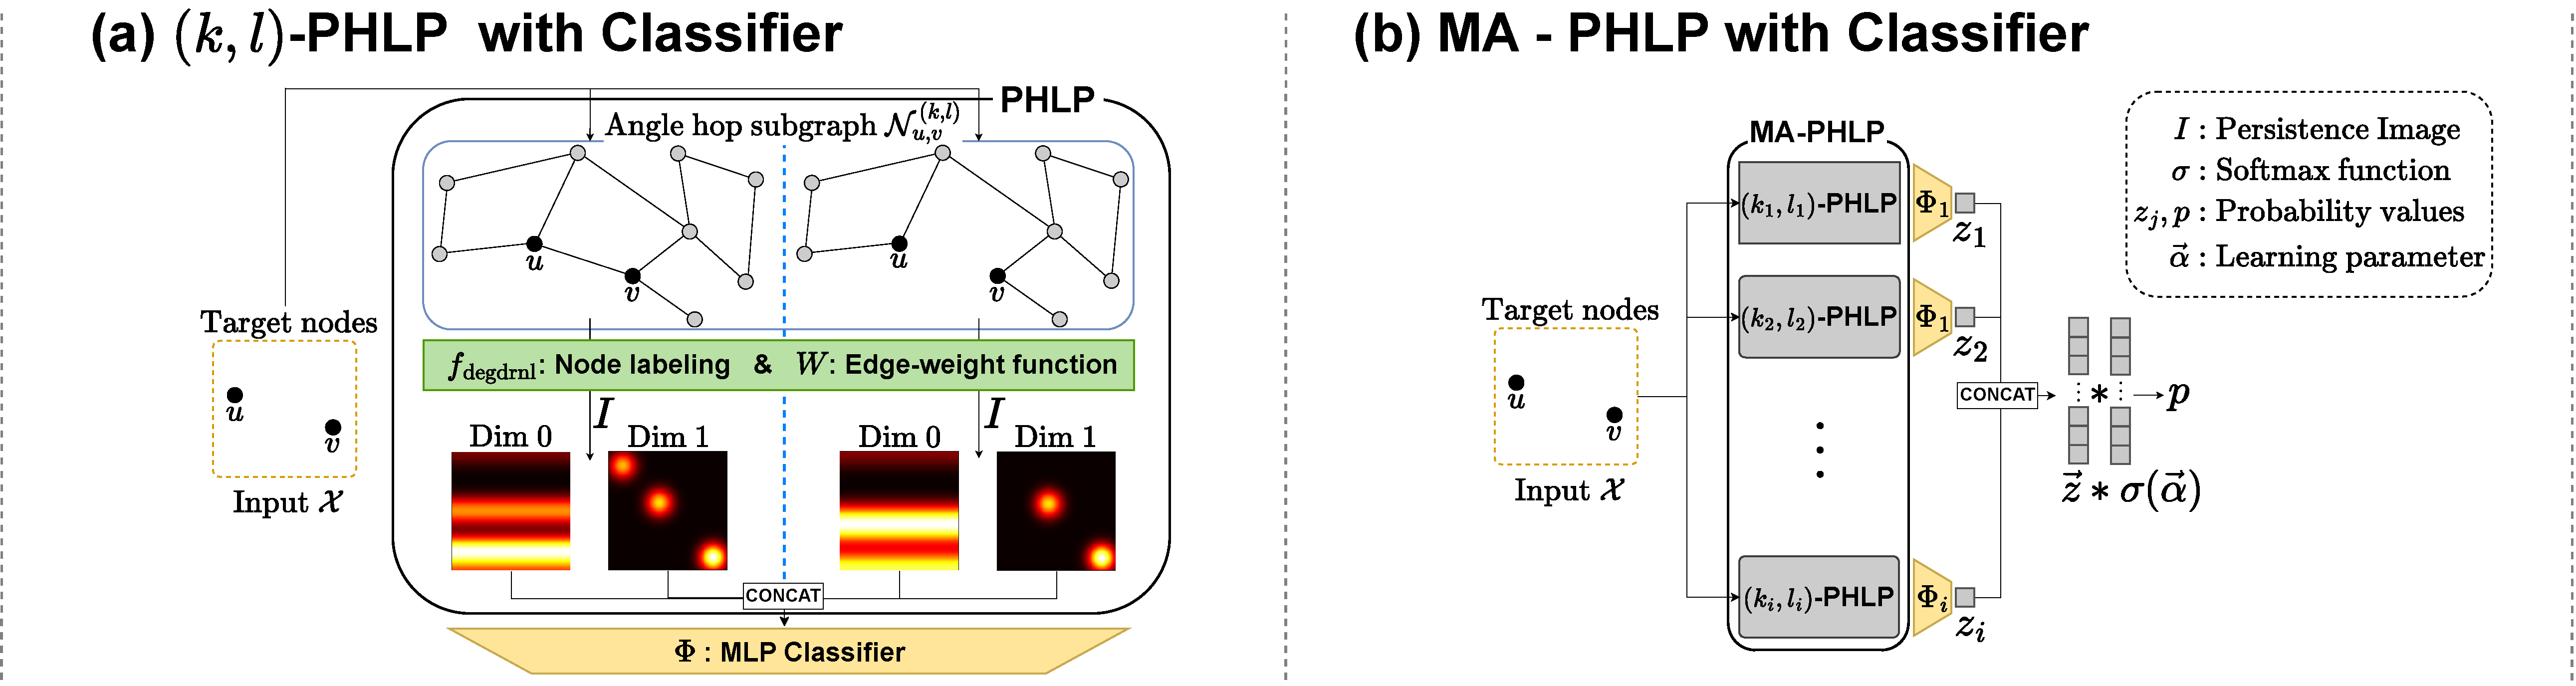
\includegraphics[width=18cm]{figures/PHLP.drawio.pdf}
\caption{Overall structure of persistent homology for link prediction (PHLP) and multiangle PHLP (MA-PHLP). (a) PHLP calculates the topological information based on the existence of target links in angle hop subgraphs for each target node. (b) With a classifier, MA-PHLP integrates topological information across various angles to perform LP. }
\label{fig:pipeline}
\end{figure*}

We propose (a) PHLP and (b) multiangle PHLP (MA-PHLP) as described in Fig.~\ref{fig:pipeline}. 
The PHLP method analyzes the topological structure of the graph, focusing on target links.
First, PHLP samples a $(k,l)$-angle hop subgraph for the given target nodes (Section~\ref{subsec:anglehop}). 
Then, PHLP computes persistence images (PIs; Section~\ref{subsec:persistenceimage}) for cases with and without the target link. 
To calculate PIs, we introduce the node labeling and define the edge-weight function (Section~\ref{subsec:filtration}).
Through PHLP, each target node is transformed into a vector comprising PIs.
In addition, LP is performed using the calculated vectors
with a classifier (Section~\ref{subsec:mlp}). 
To reflect diverse topological information, we also propose MA-PHLP, which analyzes data from various angles (Section~\ref{subsec:maphlp}).


\subsection{Extracting Angle Hop Subgraph}
\label{subsec:anglehop}

Given a graph \( G = (V, E) \) and two nodes \( u,v \in V \), a \(k\)-hop enclosing subgraph for $(u,v)$ is defined as \( \mathcal{N}^k_{u,v} = (V', E') \) such that 
\begin{align*}
    V' &= \{ z \in V \mid d(u, z) \leq k \text{ or } d(z, v) \leq k\}, \\
    E' &= \{ (z, w) \in E \mid z \in V' \text{ and } w \in V' \},
\end{align*}
where $d(z, w)$ is the minimum number of edges in any path from $z$ to $w$ in $G$.
We define a \((k,l)\)-angle hop enclosing subgraph, where the term ``angle'' signifies viewing the subgraph from multiple perspectives. 
The (k,l)-angle hop subgraph is a generalization of the $k$-hop subgraph. 
Given a graph \( G = (V, E) \) and two nodes \( u, v \in V \), a \((k,l)\)-angle hop enclosing subgraph for \( (u, v) \) is defined as \( \mathcal{N}^{(k,l)}_{u,v} = (V', E') \) such that 
\begin{align*}
    V' &= \{ z \in V \mid d(u, z) \leq k \text{ or } d(z, v) \leq l \}, \\
    E' &= \{ (z, w) \in E \mid z \in V' \text{ and } w \in V' \}.
\end{align*}
Thus, the angle hop can generate subgraphs in various forms, providing flexibility to adapt to various graph characteristics.

\subsection{Filtration of the Subgraph}
\label{subsec:filtration}

For a given subgraph, the Rips filtration~\cite{vietoris1927hoheren, gromov1987hyperbolic, edelsbrunner2002topological} is employed to calculate the topology using PH. 
To apply the Rips filtration, we define an edge-weight function using node labeling that reflects the topology of the given graph. 

\begin{figure}[!h]
\centering
\captionsetup[subfloat]{font=small}
\subfloat[\small{DRNL}]{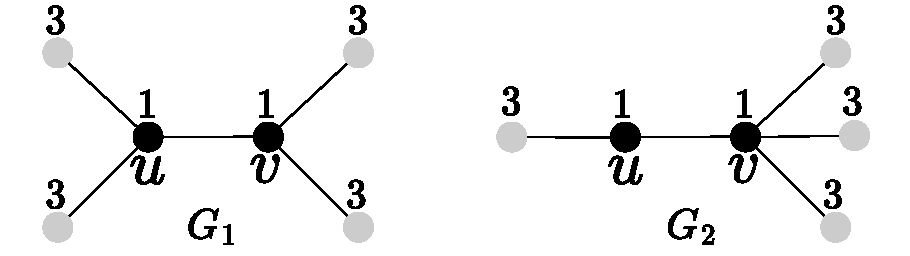
\includegraphics[width=0.9\linewidth]{figures/Drnl.pdf}
\label{drnl}}
\hfil
\subfloat[\small{Degree DRNL}]{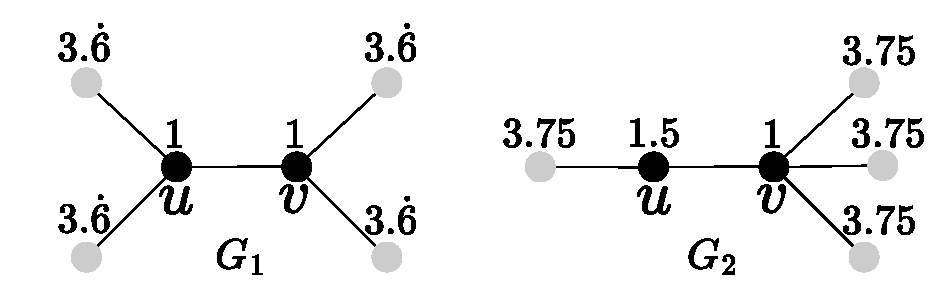
\includegraphics[width=0.9\linewidth]{figures/Degdrnl.pdf}
\label{degdrnl}}
\caption{Node labeling on graphs. (a) Node label values without considering the graph structure cannot distinguish between $G_1$ and $G_2$ using DRNL. (b) Applying Degree DRNL allows $G_1$ and $G_2$ to be distinguished solely by node label values.
}
\label{nodelabel}
\end{figure}

\begin{figure}[!h]
\centering
\captionsetup[subfloat]{font=small}
\subfloat[\small{DRNL}]{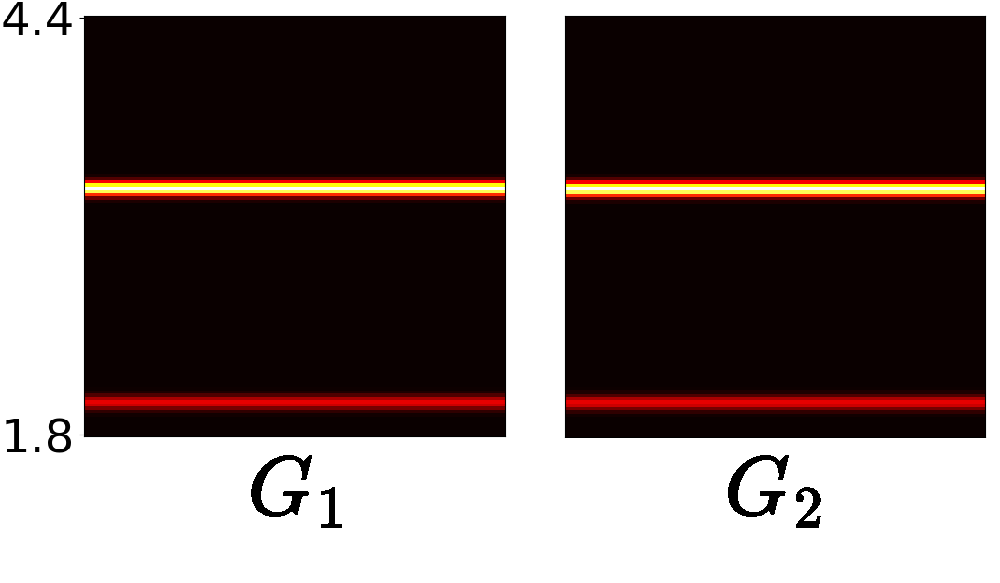
\includegraphics[width=0.48\linewidth]{figures/drnl_PI.pdf}
\label{drnl_PD}}
\hfil
\subfloat[\small{Degree DRNL}]{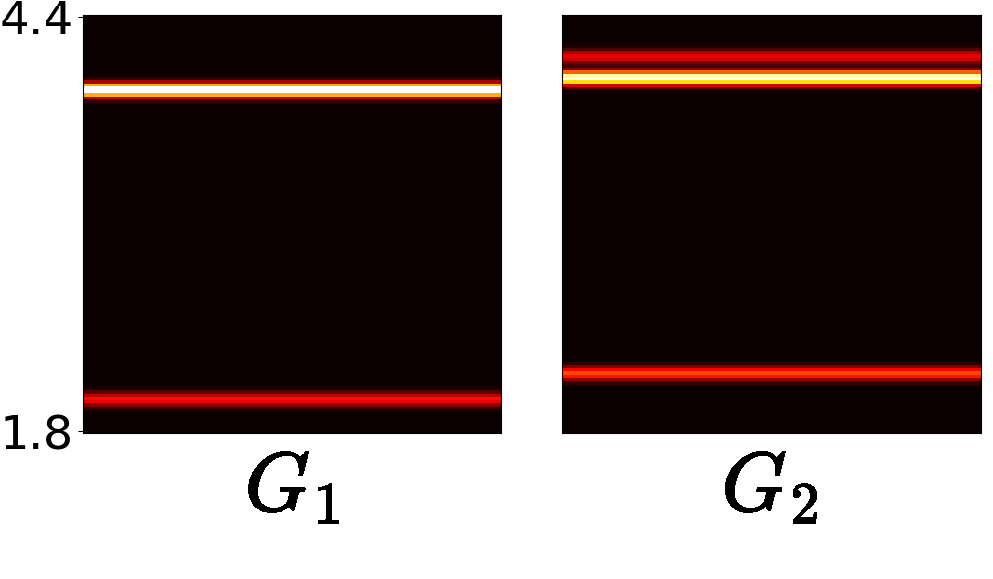
\includegraphics[width=0.48\linewidth]{figures/degdrnl_PI.pdf}
\label{degdrnl_PD}}
\caption{Persistence images (PIs) for two node labeling methods for the graphs in Fig.~\ref{nodelabel}.
(a) DRNL exhibits identical zero-dimensional PIs for $G_1$ and $G_2$, (b) Degree DRNL produces distinct outcomes, effectively distinguishing between the two.
}
\label{PD_nodelabel}
\end{figure}

\noindent\textbf{Degree DRNL.}
Zhang \textit{et al.}~\cite{zhang2018link} introduced DRNL, which computes the distance from any node to two fixed nodes.
For any subgraph $\mathcal{N}=(V',E')$ of $G$ and two nodes $a,b \in V'$, the DRNL $f^{(a,b)}_{\text{drnl}}: V' \rightarrow \mathbb{N}$ based on $(a,b)$ of $G$ for any vertex $w$ in $V'$, is defined as
\[
    f^{(a,b)}_{\text{drnl}}(w) = 1 + \min(d(w,a), d(w,b)) + q_w(q_w + r_w - 1),
\]
where $q_w \in \mathbb{Z}$ and $r_w \in \{ 0, 1\}$ are integers representing the quotient and remainder, respectively, such that $d(w,a)+d(w,b) = 2q_w + r_w$. 
We call these two nodes, $a$ and $b$, \textit{center nodes}.
These center nodes do not need to be the target nodes used when extracting the subgraph.

However, DRNL encounters limitations when the graph is transformed into node-label information.
As depicted in Fig.~\ref{drnl}, DRNL assigns the same node labels to different graphs, resulting in identical zero-dimensional PIs (Fig.~\ref{drnl_PD}, Section~\ref{subsec:persistenceimage}).
To incorporate the local topology of each node with the effects of DRNL, we introduced \textit{Degree DRNL}. 
For a given subgraph \( \mathcal{N} = (V', E') \) of $G$ and center nodes $a,b \in V'$, the Degree DRNL $f^{(a,b)}_{\text{degdrnl}} : V' \rightarrow \mathbb{R}$  based on $(a,b)$, for all vertex \( w \) in \( V' \), is defined as
\[
    f^{(a,b)}_{\text{degdrnl}}(w) = f^{(a,b)}_{\text{drnl}}(w) + \frac{M - \deg(w)}{M},
\]
where \( M \) denotes the maximum degree of nodes in \( \mathcal{N}\).
The $(M-\deg(w))/M$ term above assigns larger values for lower degrees of $w$. When $M = \deg(w)$, the value of Degree DRNL matches the original DRNL, ensuring that the edges connected to nodes with higher degrees are assigned smaller values, promoting their earlier emergence in the filtration.
Fig.~\ref{degdrnl} demonstrates various node labels obtained using Degree DRNL, resulting in PIs that can be distinguished from each other (Fig.~\ref{degdrnl_PD}). 


\noindent\textbf{Edge-weight function.} 
For a given subgraph \( \mathcal{N} = (V', E') \), \( f : V' \rightarrow \mathbb{N} \) denotes any node labeling function.
The edge-weight function $W:E' \rightarrow \mathbb{R}$, for any edge \( (w, z) \) in \( E' \), is defined as 
\[
W(w,z) =\max(f(w),f(z)) + \frac{\min(f(w),f(z))}{\max(f(w),f(z))}.
\]
The min/max term in the definition of $W$ refines values further, enhancing the discriminative power by reducing the occurrence of identical edge weights.


\subsection{Persistent Homology}
\label{subsec:persistenthomology}

Given an edge-weighted subgraph \( \mathcal{N} = (V', E', W) \), we construct a Rips filtration and compute its PH.
First, we create a sequence of subgraphs \( \{\mathcal{N}_{\epsilon}\}_{\epsilon \in \mathbb{R}} \), where each \( \mathcal{N}_{\epsilon} = (V', E'_\epsilon) \) and \( E'_{\epsilon}= \{ e \in E \mid W(e) \leq \epsilon \} \). 
Second, we convert each subgraph \( \mathcal{N}_{\epsilon} \) into the Rips complex \( K_{\epsilon} = \{ \tau \in \mathbb{X} \mid (w,z) \in E'_{\epsilon} \text{ for any two vertices } w,z \in \tau \}\), where $\mathbb{X}$ is the power set of $V'$. 
In \(K_{\epsilon}\), a simplex $\tau$ is formed when the vertices in \( \tau \) are pairwise connected by edges in \( \mathcal{N}_{\epsilon} \).
Then, the Rips filtration is obtained as \( K_{\epsilon_1} \hookrightarrow K_{\epsilon_2} \hookrightarrow \cdots \hookrightarrow K_{\epsilon_m} = \mathbb{X} \)
for $\epsilon_1 \le \epsilon_2 \le \cdots \le \epsilon_m $.
Third, we compute the $p$-dimensional homology group \( H_p(K_{\epsilon}) \) for each complex \( K_{\epsilon}\) and track how these groups change as \( \epsilon \) increases. 
The persistence diagram $D$~\cite{edelsbrunner2002topological} comprises
persistence pairs \((b,d)\) representing the \(\epsilon\) values at which a homological feature appears $b$ and disappears $d$, respectively, in the filtration.

\subsection{Persistence Image}
\label{subsec:persistenceimage}

We convert the persistence diagram into a PI~\cite{adams2017persistence}. 
For a given persistence diagram \( D \),
consider a linear transform \( L: \mathbb{R}^2 \rightarrow \mathbb{R}^2 \) defined by \( L(x, y) = (x, y-x) \). 
The image set of \( D \) under this transformation is denoted as \( L(D) \). 
For each point $(b,d')$ in $L(D)$, a weight function \( \phi_{(b,d')}: \mathbb{R}^2 \rightarrow \mathbb{R} \) is defined that assigns a weight to each point in the persistence diagram. 
A common choice for \( \phi_{(b,d')} \) is the Gaussian function centered at $(b,d')$.
The nonnegative function is defined as $h:\mathbb{R}^2 \rightarrow \mathbb{R}$, as $h(x,y)=1/\log(1+ \lvert y \rvert)$.
The function $h$ is zero along the horizontal $x$-axis, and is continuous and piecewise differentiable, satisfying the conditions presented in~\cite{adams2017persistence}.
The persistence surface $\rho_D:\mathbb{R}^2 \rightarrow \mathbb{R}$ is defined as
\[
\rho_D(z) = \sum_{(b,d') \in L(D)} h(b,d')\phi_{(b,d')}(z).
\]

The continuous surface \( \rho_D \) is discretized into a finite-dimensional representation over a predefined grid. 
This grid consists of \( n \) cells, each corresponding to a specific region in the plane. 
The PI is defined as an array of values \( I(\rho_D)_p \) for each cell $p$. 
Each $I(\rho_D)_p$ in this array is computed by integrating the persistence surface \( \rho_D \) over the area of cell $p$:
\[
 I(\rho_D)_p  = \iint_{p} \rho_D \, dy \, dx.
\]

\subsection{Predicting the Existence of the Target Link}
\label{subsec:mlp}
For the given target nodes $(u,v)$, we sample the $(k,l)$-angle hop subgraph \( \mathcal{N}^{(k,l)}_{u,v}\), denoted as \(\mathcal{N}^-\) (Section~\ref{subsec:anglehop}), assuming that the target link does not exist during this process. 
On this subgraph, we extract topological features by calculating PH and its vectorization (i.e., the PI, as described in Sections~\ref{subsec:persistenthomology} and~\ref{subsec:persistenceimage}). The vectorization is calculated for each dimension and concatenated. If $k \neq l$, for symmetry, we repeat the same process with the $(l,k)$-angle hop subgraph once and consider the average of the two vectors, denoting this vector as $x^-$. 
To observe the difference in topological features, we consider a subgraph \( \mathcal{N}+ \) obtained by connecting the target link to \(\mathcal{N}^-\).
For this graph, \(x^+\) denotes the vector obtained using this method.

To predict the existence of the target link with the vectors \(x^-\) and \(x^+\), we employ an MLP classifier $\Phi: \mathbb{R}^{2(d+1)n^2} \rightarrow \mathbb{R}$ where $n$ represents the resolution of the PI, and $d$ denotes the maximal dimension of PH. 
The model predicts the existence of a link between two target nodes with the following probability: 
\[
    z_{uv} = \sigma(\Phi(x)), 
\]
where $x$ is the concatenation of $x^-$ and $x^+$, and $\sigma$ is the activation function.
For the training dataset \(\mathcal{X} \subseteq V \times V\), comprising positive and negative links corresponding to the elements of \(E\) and \((V\times V)\setminus E\), respectively, we define the loss function as follows:
\[
    \sum_{(u,v) \in \mathcal{X}} BCE(z_{uv}, y_{uv}),
\]
where \(BCE(\cdot,\cdot)\) represents the binary cross-entropy loss and \(y_{uv}\) denotes the label of the target link \((u,v)\), which is \(0\) for negative links or \(1\) for positive links.

\subsection{Multiangle PHLP}
\label{subsec:maphlp}
The MA-PHLP maximizes the advantages of PHLP by examining data from various angles through the extraction of subgraphs based on a hyperparameter, the maximum hop (max hop, denoted as $H$).
The types of angles are elements of all combinations of \(k\) and \(l\) within the set \(\{(k,l) \in \mathbb{Z}^2 | 0 \leq l \leq k \leq H, k > 0\}\).
If we define the prediction probability of a PHLP for each type of angle hop as $z_i$ for $i=1, 2, ..., N$, then MA-PHLP predicts the likelihood of the link existence with the following probability: 
$$p = \sum_{i=1}^N \alpha_iz_i ,$$
where $\alpha = (\alpha_1,...,\alpha_N) \in \mathbb{R}^N$ is a trainable parameter.
We apply the softmax function to the parameter \(\alpha\) to ensure that the sum of all elements equals $1$. 
Moreover, MA-PHLP is trained using the binary cross-entropy loss.

\subsection{Hybrid Method}
\label{subsec:hybrid}
The proposed approach easily integrates with existing subgraph methods. Subgraph methods treat the LP task as a binary classification problem comprising two components: a feature extractor $F$ and classifier $P$. Vectors with PH information calculated using the proposed methods are incorporated through concatenation before the classifier.
The detailed process of the hybrid method is outlined as follows: 
\begin{enumerate}
    \item \textbf{Subgraph Extraction:} For the given graph $G$ and target nodes $(u,v)$, $k$-hop subgraph $\mathcal{N}^k_{u,v}$ is extracted. 
    \item \textbf{Feature Extraction:} Existing methods extract features $Z = F(\mathcal{N}^k_{u,v})$ from the subgraph.
    \item \textbf{Persistent Image Calculation:} The methods described in Sections~\ref{subsec:filtration}, \ref{subsec:persistenthomology}, and~\ref{subsec:persistenceimage} are applied to $\mathcal{N}^k_{u,v}$, where $I$ denotes the PI vector. An MLP $\Phi:\mathbb{R}^m \rightarrow \mathbb{R}^n$ transforms the PI into a format similar to $Z$. 
    For the hybrid method of MA-PHLP, $\mathcal{N}^k_{u,v}$ is replaced with multiangle subgraphs, concatenating their PI vectors.
    \item \textbf{Classification:} Next, $\alpha_1 Z$ and $\alpha_2 \Phi(I)$ are concatenated, where $\alpha_1$ and $\alpha_2$ are trainable parameters. The softmax function is applied to the parameter \(\alpha=(\alpha_1,\alpha_2)\), ensuring that the sum of elements equals $1$, denoted by $J$.
    This concatenated vector is classified using the existing method's classifier, $P(J)$.
\end{enumerate}